\begin{kwote}
``Qu'elle suive des normes ou pas, la réflexion sur l'interface, sur le
rendu graphique d'un projet de recherche devrait être présente dès
l'origine du processus. Cela demande, comme pour la gestion des
métadonnées, une attitude en apparence paradoxale mais nécessaire pour
mener un projet de recherche aujourd'hui~: l'anticipation des
problématiques de valorisation dès l'amont du projet.''\footcite{jacquot_decrire_2017}
\end{kwote}

Cette affirmation souligne l'importance d'une interface utilisateur.rice
intuitive et performante, non seulement pour favoriser
l'adoption d'un outil par la communauté scientifique, mais aussi pour
prévoir la valorisation des résultats de recherche. Les décisions
techniques liées à l'interface répondent ainsi à un double objectif~:
fournir aux chercheur.ses un environnement de travail, et faciliter la diffusion et la médiation des données de la
recherche auprès d'un public de non-spécialistes, anticipant la création
d'une plateforme publique.

\hypertarget{interface-admin-django}{%
\subsection{Interface Admin Django vs. vues personnalisées}\label{interface-admin-django}}

Une fonctionnalité puissante et intéressante de Django est son interface
d'administration automatique, qui a servi d'interface à \eida dans un
premier temps. Cette interface lit les métadonnées du modèle pour
fournir rapidement un outil de gestion centrée sur celui-ci. Via cette
interface \textit{backend} les utilisateur.rices administrateurs peuvent gérer les
contenus du site. Cependant, son utilisation est limitée à des fins de
gestion interne et ne suffit pas pour servir de base à la création d'une
interface distribuable ou publique. Cette fonctionnalité est pertinente
si une interface centrée sur les tables et les champs de base de données
est nécessaire. Cependant, pour une interface qui fait abstraction des
détails d'implémentation de la base de donnée, centrée davantage autour
des processus, l'interface d'administration automatique de Django
devient insuffisante et il faut construire des vues personnalisées.

La construction d'une vue dans Django passe par l'écriture d'un template
\html dans lequel le python injectera les données structurées par une
fonction définie dans le fichier \texttt{view.py}. Le fichier \texttt{urls.py} est aussi
un composant essentiel du \textit{framework}. Il sert à définir les mappages
entre les \URLs des requêtes entrantes et les vues correspondantes. En
d'autres termes, il gère le routage des requêtes \http en les dirigeant
vers les fonctions qui traiteront ces
requêtes, faisant elles-mêmes l'intermédiaire entre les données et leur affichage.

Écrire des vues dans Django sans utiliser de \textit{framework} \emph{front-end} génère
donc directement le \html à partir des \textit{templates}. Les interactions
utilisateur.rice sont gérées par des requêtes \http traditionnelles. Ce mode
de développement, simple et rapide à mettre en place, est
particulièrement adapté pour des applications avec des interactions
limitées ou des besoins modérés en termes de dynamisme. Dans l'interface \eida, il a
permis la création de vue personnalisées et adaptées aux visualisation
des sorties de l'inférence avec les modèles d'extraction, de similarité
et de vectorisation. La description de certains de ces développements est présentée en annexe \ref{dvt_interfaces}. 

Au mi-terme de mon stage, a été prise la décision de refondre les
interfaces et d'adopter un \emph{framework front-end}, offrant une
expérience utilisateur.rice plus fluide grâce à une gestion différente des
interactions entre le \textit{back-end} et le \textit{front-end}.

\hypertarget{utilisation-dun-framework-front}{%
\subsection{Utilisation d'un \emph{framework
front}}\label{utilisation-dun-framework-front}}

\begin{kwote}
``La structure de l'application ainsi que l'architecture client/serveur
conditionnent la manière dont est traitée l'information. Ainsi, pour
assurer aux internautes une expérience de navigation agréable au sein du
front office, les problématiques de vitesse de chargement doivent
influencer directement la manière dont sont pensés les développements.
S'il est préférable d'effectuer la manipulation de données dans la
partie back-end de la plateforme, il est cependant nécessaire de savoir
repenser les méthodes de requêtage et de gestion des données, afin
d'offrir aux utilisateur.rices des interfaces optimales et
ergonomiques.''\footcite[p.97]{albouy_mediation_2019}
\end{kwote}

Pour les applications web utilisant le protocole \http lors d'une action
de l'utilisateur.rice, le contenu de la vue est recalculé puis envoyé au
client. Or, pour la manipulation d'ensembles de données lourds dans une
même interface, il est intéressant d'avoir recours à des méthodes de
programmation asynchrone au sein du \textit{front-end}, de façon à réduire les
durées de chargement à l'ouverture de la page.

Les \textit{frameworks} \textit{front-end} sont des collections de ressources (fichiers,
bibliothèques, structures de code, etc.) permettant de créer une
interface utilisateur.rice plus dynamique et réactive, essentiellement pour
les applications nécessitant une manipulation de contenus visuels,
offrant ainsi une expérience utilisateur.rice plus fluide et agréable. Ils
sont conçus pour optimiser les performances en gérant efficacement le
\dom et en permettant des mises à jour en temps réel sans recharger la
page entière. De plus, grâce à la virtualisation des données et à la
manipulation asynchrone, ils permettent de charger et de rendre les
données lourdes de manière progressive, réduisant ainsi les temps de
latence et améliorant la réactivité globale. Par ailleurs, ils vont
faciliter l'adoption de normes et standards pour le développement de la
partie frontale, donnant un rendu plus unifié.

Pour comprendre le fonctionnement d'un tel outil, une digression
s'impose à propos de l'architecture client/serveur, sur laquelle repose les
applications web.

\hypertarget{paradigme-clientserveur-back-endfont-end-spa}{%
\subsubsection{Paradigme client/serveur~; \emph{back-end}/\emph{font-end}~;
SPA}\label{paradigme-clientserveur-back-endfont-end-spa}}

L'architecture client/serveur définit le mode de communication entre
deux programmes~: le client, qui envoie des requêtes, et le serveur, qui
y répond. Dans une plateforme en ligne, le serveur envoie les pages
affichées sur le navigateur du client, et le client (utilisateur.rice) envoie
des requêtes au serveur en agissant sur l'interface.

Cette architecture se reflète dans la distinction entre le développement
\textit{back-end} et \textit{front-end}. Le \textit{back} concerne la partie du code invisible à
l'utilisateur.rice (par exemple, en Python pour \eida), tandis que le \textit{front}
concerne la partie visible, influençant directement ce qui est affiché à
l'écran (en \html, \textsc{css} et JavaScript). Le code Python est exécuté sur le
serveur, tandis que le \html, \textsc{css} et JavaScript sont interprétés par le
navigateur du client.

Les méthodes de traitement des données varient~: le serveur, souvent
plus puissant, exécute plus rapidement les procédures lourdes en Python.
C'est pourquoi les données sont formatées en \textit{back-end} avant de les
transmettre eu \textit{front-end}. Toutefois, ce mode de traitement des
ressources peut être optimisé pour certaines situations. Les méthodes
dites asynchrone effectuent des traitement en \textit{front-end}, afin de réduire
les temps de chargement et de fluidifier l'expérience utilisateur.rice.
JavaScript récupère des données du serveur sans entraver l'exécution du
reste du code. Cette technique permet au navigateur de continuer à
fonctionner de manière fluide et réactive, même lorsqu'il attend une
réponse du serveur. Lorsqu'une requête asynchrone est envoyée,
JavaScript utilise des \apis telles que Fetch ou XMLHttpRequest pour
interagir avec le serveur en arrière-plan. Une fois la réponse du
serveur reçue, une fonction de rappel (callback) ou une promesse
(promise) traite les données retournées sans avoir interrompu les
opérations en cours. Cette approche est largement utilisée par les
applications web modernes, permettant une mise à jour dynamique du
contenu et une meilleure expérience utilisateur.rice, en évitant les temps
d'attente et les blocages qui pourraient survenir avec des requêtes
synchrones traditionnelles~: on les nomme \spa, par opposition aux \mpa classiques.

Une \spa est une application web qui charge
une seule page \html et met à jour dynamiquement le contenu au fur et à
mesure que l'utilisateur.rice interagit avec l'application. Lors du
chargement initial, le serveur envoie les fichiers \html, \textsc{css} et
JavaScript nécessaires. La page \html chargée inclut des zones réservées
(comme des éléments \texttt{div}) où le contenu sera remplacé dynamiquement. Les \spa utilisent
généralement des \textit{frameworks} JavaScript tels que React, Angular, Vue.js
ou Svelte qui gèrent le rendu du contenu directement dans le navigateur,
sans dépendre du côté serveur. À mesure que l'utilisateur.rice interagit avec
l'application (par exemple, en cliquant sur des liens ou des boutons),
le \textit{framework} intercepte ces actions et charge de nouveaux contenus ou
données de manière asynchrone. Ce processus se fait souvent en
effectuant des appels \api pour récupérer des données d'un serveur ou
d'une base de données. Lorsque de nouvelles données sont récupérées, le
\textit{framework} met à jour le \dom de manière dynamique sans recharger la page
entière (Fig.\ref{fig:spa}).

        \begin{figure}[H]
          \begin{center}
          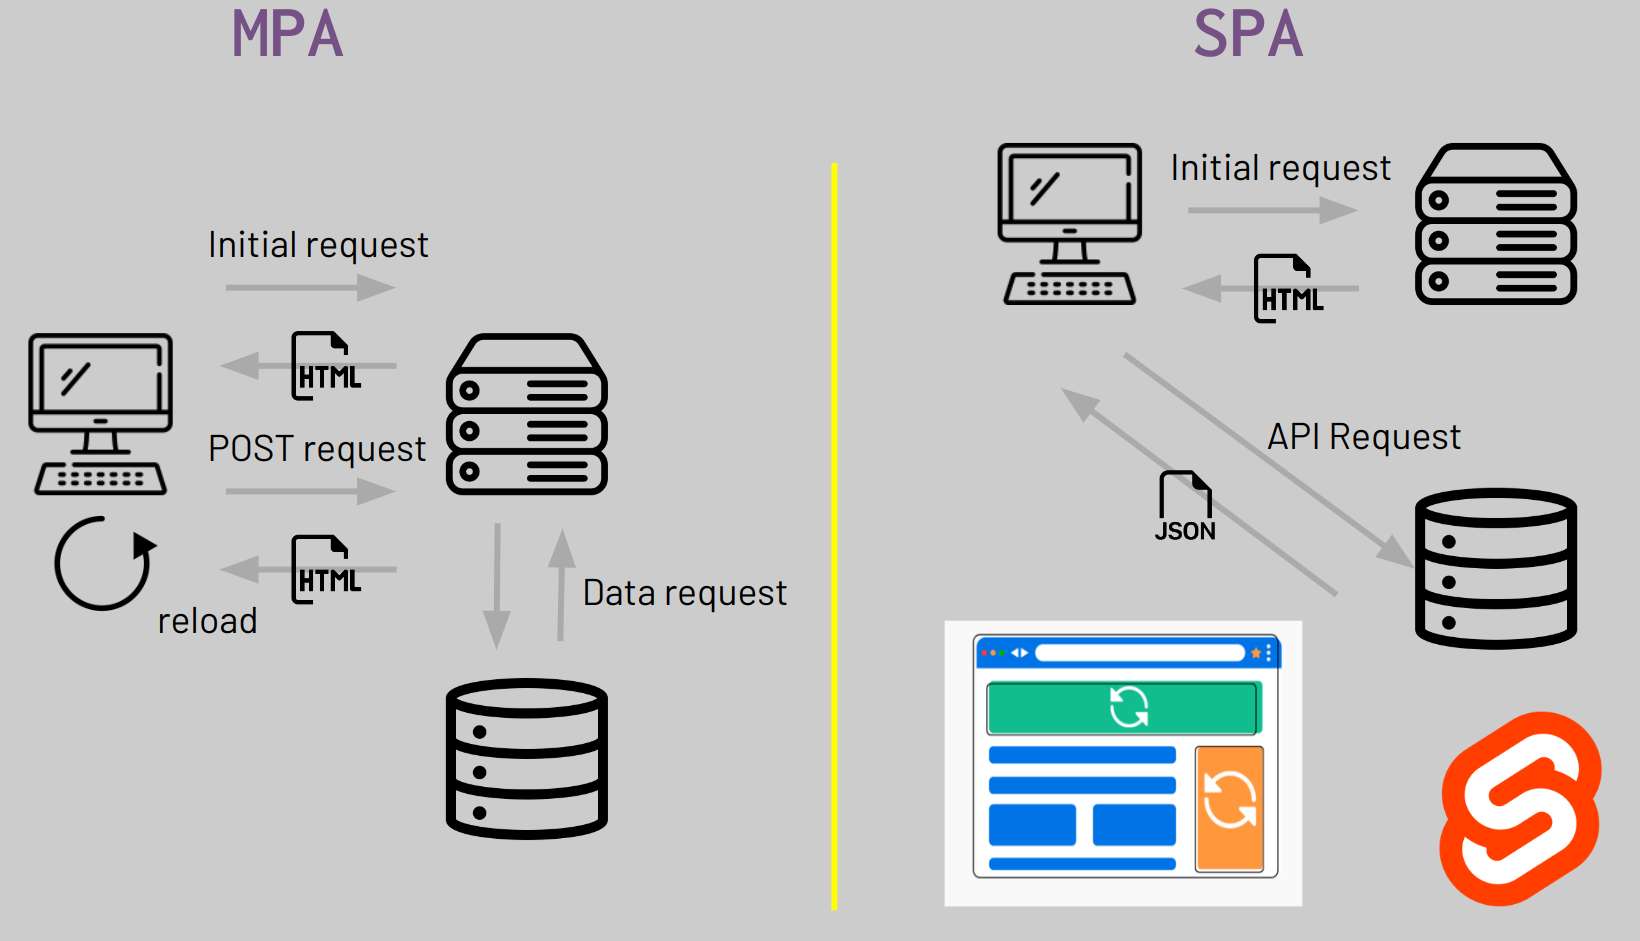
\includegraphics[height=6cm]{figues/SPA.png}
          \end{center}
          \caption{Fonctionnement schématique d'une \spa.}
          \label{fig:spa} \end{figure}

Leur mode de fonctionnement donnent aux \spa rapidité et fluidité~: après
le chargement initial, elles ne récupèrent et ne rendent que le contenu
qui doit être mis à jour, plutôt que de recharger toutes les ressources
chaque fois que l'utilisateur.rice interagit avec l'application.

\aikon n'est pas une \spa. C'est une application classique qui donne à
certaines pages le fonctionnement d'une \spa, pour permettre plus
d'interaction en conservant fluidité et performance. Cela est possible
grâce à l'utilisation de requêtes asynchrones, permises par l'adoption
d'un \textit{framework front-end}~: Svelte, ajouté de manière incrémentielle à la
base de code existante.

\hypertarget{svelte}{%
\subsubsection{Svelte}\label{svelte}}

Pour gérer efficacement un volume de contenu visuel et éviter le temps
de latence au chargement de certaines pages, \aikon s'appuie donc sur des
requêtes asynchrones et sur Svelte.js, choisi pour ses performance.

Une page construite avec Svelte est à considérer comme un ensemble de
\textit{Components} (composants), unités de code réutilisables et
auto-suffisantes. Les composants sont écrits en utilisant la
\emph{Svelte syntax}, un langage propre à Svelte~: il reprend les trois
langages de base \html, \textsc{css} et JavaScript, mais sans les diviser. On les
retrouve tous les trois dans les mêmes fichiers (en gardant une base de
\html~: c'est avant tout un langage de balisage). Le développement est
alors moins verbeux, et le langage est plus simple et lisible, et donc
plus maintenable.

Svelte est davantage un compilateur qu'une \textit{Library}, c'est ce qui le
distingue et optimise ses performances. Ce nouveau paradigme permet une
répartition optimisée du travail entre le serveur et le client.
Contrairement à d'autres \textit{frameworks front-end}, avant que le code Svelte
ne soit chargé dans le navigateur, il passe par une étape de compilation
en JavaScript pur côté serveur, lors de la phase dite de \textit{build}. Le
code Svelte, écrit avec sa syntaxe propre, est transformé en JavaScript
\emph{vanilla}, très performant\footnote{Le JavaScript \textit{vanilla}, ou
  JavaScript pur, désigne l'utilisation du langage JavaScript sans
  recourir à bibliothèques ou \textit{frameworks} externes. C'est la forme de
  JavaScript la plus fondamentale, directement intégrée dans les
  navigateurs web, permettant d'écrire des scripts légers et performants
  pour interagir avec le \dom et réaliser diverses fonctionnalités côté
  navigateur.}. Le code exécuté dans le navigateur est léger, rapide et
optimisé, puisqu'il n'y a pas de \textit{framework} lourd à exécuter~; et
l'expérience utilisateur.rice en est d'autant plus fluide.

L'étape de compilation permet aussi d'intégrer la réactivité directement
dans le langage. Chaque variable déclarée dans un composant Svelte est,
par défaut, un objet réactif. Lorsqu'une nouvelle valeur est affectée à
cette variable (via \texttt{=}, \texttt{+=}, \texttt{-=}, ou
\texttt{\$}\footnote{L'opérateur \texttt{\$} assigne une variable à une
  autre non déclarée, à cette dernière Svelte ajoutera automatiquement
  une déclaration \texttt{let}, et entre les deux se crée une
  dépendance, un lien durable. Où que la première variable change dans
  le code, le changement sera détecté et affectera la seconde. Svelte
  crée ainsi une sort d'arbre des dépendances insensible à l'ordre des assignations.}), Svelte
ne se contente pas d'effectuer une simple assignation. Il surcharge les
opérateurs d'un appel à une sorte de fonction, un effet de bord, généré par
le compilateur, qui va détecter les dépendances (identifier tous les
éléments du \dom ou autres expressions qui dépendent directement ou
indirectement de cette variable), et mettre à jour le \dom (planifier une
mise à jour de ces éléments afin d'afficher le nouvel état à l'écran).

\begin{kwote}
``Updating some count value --- and all the things that depend on it ---
should be as simple as this:

\texttt{count\ +=\ 1;}

Since we're a compiler, we can do that by instrumenting assignments
behind the scenes:

\begin{verbatim}
count += 1;
$$invalidate('count', count);
\end{verbatim}

Importantly, we can do all this without the overhead and complexity of
using proxies or accessors. It's just a variable.''\footcite{harris_svelte_2019}
\end{kwote}

Cette approche permet de se passer de \dom virtuel. Le \textit{virtual \dom} est un
objet JavaScript, une copie de l'arbre des composants (le vrai \dom,
celui qui est interprété et rendu dans le navigateur), utilisé par le
plupart des autres \textit{framework} front comme React.js, Angular.js ou
Vue.js. À chaque trame de rendu, le \textit{framework} compare un à un les
paramètres de chaque nœud de l'arbre des composants entre la copie de
l'ancien (\textit{virtual \dom}) et le nouveau \dom. S'il y a un paramètre à
changer, le \textit{framework} ne rafraîchit le rendu que des nœuds qui en
dépendent. Mais cette comparaison des nœuds un à un est coûteuse. Svelte
suit directement les dépendances entre valeurs uniquement grâce au
langage. Lorsque une donnée change, Svelte sait exactement quels
éléments de l'interface doivent être mis à jour, sans avoir à parcourir
l'ensemble de l'arbre des composants. Ce paradigme permet plus
d'efficience et améliore la réactivité.

Les composants Svelte sont conçus pour être autonomes et indépendants.
Cependant, il est fréquent de devoir partager des données entre
plusieurs composants. C'est là qu'interviennent les \textit{stores}. Un \textit{store}, en
Svelte, est un objet indépendant de la hiérarchie des composants (il est
typiquement déclaré en dehors de tout composant, dans un fichier
séparé), qui contient les variables avec leur état, et permet leur
partage entre différents \textit{Components}. Il fonctionne comme un dépôt
centralisé où la donnée est stockée et mise à jour. Les composants qui
ont besoin d'accéder aux données d'un store s'y ``abonnent''. Lorsque la
valeur d'une variable dans un store est modifiée, le changement est
automatiquement propagé et tous les composants abonnés sont mis à jour,
affichant alors le nouvel état des données à l'écran. L'état de
l'application est géré de manière centralisée, ce qui améliore la
lisibilité du code.

Dans le cas d'\aikon, où l'interface utilisateur.rice doit gérer de manière
dynamique un grand nombre d'images et de filtres complexes, Svelte s'est
avéré un choix judicieux. La capacité de Svelte à mettre à jour
l'interface en temps réel, en réponse aux actions de l'utilisateur.rice,
comme l'application de filtres sur les résultats de recherche de
similarité, permet de conserver la fluidité dans l'interaction. Les
multiples critères de filtrage -- témoins à comparer, catégories de
similarité -- et leur interdépendance -- les catégories à afficher
reposent sur la catégorisation apposée à chaque image -- rendent
l'interface particulièrement dynamique, et Svelte permet la gestion de
cette complexité.

Essentiellement, Svelte reprend l'idée d'une \spa pour développer toute
ou une partie d'une interface. Il propose cependant une alternative
intéressante aux \textit{frameworks front-end} traditionnels. En compilant le
code à la volée et en générant du JavaScript pur, Svelte offre un
optimisation du temps de latence, notamment pour le développement
d'applications web qui restent réactives malgré le volume de données.

\hypertarget{le-design-dinterface}{%
\subsection{Le design d'interface}\label{le-design-dinterface}}

La dernière étape de l'\ux/\ui \textit{design} consiste à travailler sur le rendu
visuel du produit afin que l'interface soit claire, lisible, attrayante
et simple d'utilisation. Il s'agit par exemple de choisir la bonne
couleur afin de rendre un bouton visible, choisir la bonne police pour
plus de lisibilité, etc. 

Un \textit{framework \textsc{css}} est une bibliothèque pré-conçue de fichiers \textsc{css} qui
permettent de simplifier et standardiser le développement de la mise en
page et du design des sites web. Ces \textit{frameworks} fournissent des outils,
des styles, et des composants réutilisables pour créer des interfaces
utilisateur.rice de manière plus efficace et cohérente. Notamment, ils
simplifient l'obtention d'un résultat \textit{responsive}, s'adaptant à
différents mode d'affichage et plusieurs écrans. Pour le développement
de la plateforme, Bulma a été utilisé.

En outre, l'utilisation des fonctionnalités avancées comme les fonctions
ou les variables personnalisables, permettent aux développeur.ses de créer
des styles plus dynamiques, et surtout réutilisables, ce qui est
particulièrement pertinent dans le cadre du développement collaboratif
afin d'aligner la charte graphique.

Les variables personnalisées sont définies à l'aide du préfixe
\texttt{-\/-} et peuvent être réutilisées dans tout le document \textsc{css}.
Elles permettent de centraliser la gestion des couleurs et d'autres
valeurs répétitives. Par exemple, il est possible de définir une couleur
que prendront les éléments au survol grâce à son code hexadécimal ou les
valeurs RGB, en lui assignant un nom (\texttt{-\/-on-hover}). La
variable sera alors réutilisable avec la même facilité que les variables
de couleur intégrées dans Bulma (comme \texttt{-\/-bulma-danger-light}).

Il est aussi possible d'assigner des variables par défaut~:

\begin{lstlisting}[language=css, frame=single, breaklines=true, caption={Créations de variables \textsc{css} personnalisées.}]
:root {
    --bulma-body-family: "Fira Sans", sans-serif;
    --default-color: hsl(229, 68%, 46%);
    --accent-grey: hsl(0, 0%, 14%);
\end{lstlisting}

Utiliser la pseudo-classe \texttt{:root} pour définir des variables \textsc{css}
garantit qu'elles sont accessibles partout dans le document, en
utilisant la fonction \texttt{var()}, comme ci-dessous~:

\begin{lstlisting}[language=css, frame=single, breaklines=true, caption={Utilisation de variables \textsc{css} personnalisées.}]
.navbar-link:hover {
    background-color: inherit;
    color: var(--default-color);
}
\end{lstlisting}

Pour aller plus loin dans la standardisation, il est possible de définir
des styles thématiques.

\begin{lstlisting}[language=css, frame=single, breaklines=true, caption={Définition d'un thème sombre et d'un thème claire grâce aux classes \textsc{css}.}]
[data-theme="light"] {
    --contrasted: #f3eff1;
    --accent: hsl(0deg 0% 0% / 5%);
    --selected: hsl(234deg 100% 96%);
    --selected-text: hsl(237deg 82% 32%);
    --deleted: var(--bulma-danger-light);
    --deleted-text: var(--bulma-danger-dark);
}

[data-theme="dark"] {
    --contrasted: #252424;
    --accent: hsla(0, 0%, 100%, 0.05);
    --selected: #000528;
    --selected-text: #7281f9;
    --deleted: var(--bulma-danger-dark);
    --deleted-text: var(--bulma-danger-light);
\end{lstlisting}

Dans l'exemple ci-dessus, des variables personnalisées sont utilisées
pour définir un mode clair et un mode sombre. Les styles sont appliqués
en fonction de l'attribut \texttt{data-theme} sur un élément \html
(\texttt{\textless{}body\ data-theme="light"\textgreater{}} ou
\texttt{\textless{}body\ data-theme="dark"\textgreater{}}). Cela permet
de basculer facilement du mode sombre au mode clair, sans redéfinir les
modalités du changement dans chaque élément affecté.

Les \textit{media queries} sont des techniques \textsc{css} qui permettent d'appliquer des
styles en fonction des caractéristiques du périphérique sur lequel le
contenu est affiché, comme la largeur de l'écran, la résolution, ou dans
le cas illustré ci-dessous, la préférence du schéma de couleurs de
l'utilisateur.rice.

\begin{lstlisting}[language=css, frame=single, breaklines=true, caption={Utilisation des \emph{media queries}.}]
@media (prefers-color-scheme: dark) {}
@media (prefers-color-scheme: light) {}
\end{lstlisting}

En somme, le design d'interface rend l'expérience de l'utilisateur.rice plus
agréable en prenant en compte ces préférences d'affichage (mode ou
taille d'écran) et en offrant une identité visuelle cohérente. Il
contribue à l'adoption des outils au sein des équipes de recherche. Par
ailleurs, l'utilisation d'un \textit{framework \textsc{css}} rationalise le développement
\textit{front-end}, simplifiant le travail de l'équipe de développement, qui
peut alors de se concentrer sur les fonctionnalités clés plutôt que
sur des aspects purement esthétiques.